\documentclass[10pt,journal,compsoc]{IEEEtran}

\usepackage[pdftex]{graphicx}    
\usepackage{cite}
\usepackage{listings}
\usepackage{subcaption} 
\usepackage{dirtree}
\hyphenation{op-tical net-works semi-conduc-tor}
\graphicspath{ {../images/} }


\begin{document}
	
\title{Robotics Software Engineer Nanodegree: Inference Project}
\author{Manuel Huertas L\'opez}

\markboth{Inference project, Udacity}{}
\IEEEtitleabstractindextext{%
	
\begin{abstract}
This project consists of two parts. In the first part of the project a data set is provided, and a Neural Network must be trained in order to achieve an inference time less than 10 ms and accuracy greater than 75\%. In the second part of the project an original idea for a robotic inference system must be selected; them the data must be collected and a network trained. The project selected, identify and classify coins, has been taking into account that, in a robotic system we want to perceive the world, make a decision based on that perception, and them act upon this decision. The Neural Network may have several real world applications: automate the process of counting coins, help blind people in everyday situations and so on.
\end{abstract}


\begin{IEEEkeywords}
inference project, udacity, deep learning.
\end{IEEEkeywords}}
	
	
\maketitle
\IEEEdisplaynontitleabstractindextext
\IEEEpeerreviewmaketitle
\section{Introduction}
\label{sec:introduction}
\IEEEPARstart{T}{he} field of robotics has evolved during the last decades. During the industrial revolution, the robots that were manufactured could operate repetitively with high precision. The current robots can move around the scene detecting automatically obstacles and reacting in real time to changes in the environment. The flexibility needed for the new era of robots can be beneficed of the neural networks applied to image classification or semantic segmentation. By using these techniques a trained robot can rapidly identify objects in the scene and react accordantly.  It is not only provided with sensors to avoid obstacles, it can detect object in the scene, classified them, and to make decision bases on this classification.

In addition, the use of neural network can be extended to days basis. Nowadays, a lot of people posses a mobile with the capabilities to carry on inference task. The range for applications that can be developed for these platforms is huge with the only limitation of the imagination.

A lot of effort to provide the robots these capabilities cames from collecting data to train the Neural Network and to define the network architecture itself. In the present work an example, classify coins, have been selected in order to evaluate the data collection process and the architecture selection and finally, to do the verification.
	
\section{Background / Formulation}

\subsection{Udacity}

The Udacity provided data set, to be classified by the Neural Network, consists of a collection of objects of three types: candy boxes, bottles and nothing.

GoogleNet network was selected for several reasons \cite{analysisdnn}:

\begin{enumerate}
\item The image size fits well with one required by the network.
\item The network gives enough accuracy to pass requirements.
\item The number of operations, that is related to the inference time, is around 3 G-ops.
\end{enumerate}


A classification network was selected with the following parameters:

\begin{itemize}
	\item Training epochs[5]: how many passes throught the training data.
	\item Standard Network[GoogLeNet]: the predefined network achitecture.
\end{itemize}


\subsection{Original Idea}

The original idea selected was identified a coin in an image and to classify the coin, three different kinds of classes were used, corresponding to the European coins of 10 cents, 20 cents and one Euro.

GoogleNet network was selected for several reasons \cite{analysisdnn}:

\begin{enumerate}
	\item The image size fits well with one required by the network.
	\item The network gives a good accuracy with a reasonable inference time.
	\item The network uses color image. For the Euros to be identify it is quite useful.
	\item The number of operations, that is related to the inference time, is around 3 G-ops.
\end{enumerate}

A classification network was selected with the following parameters:

\begin{itemize}
	\item Training epochs[5]: how many passes throught the training data.
	\item Standard Network[GoogLeNet]: the predefined network achitecture.
\end{itemize}

		
\section{Data Acquisition}

The data set was collected using the camera of a mobile phone. The coins were put on a white paper and a video recording was started. Every few seconds the recording was paused to turn the coin randomly. Then, a tool to extract individual images from the video, ffmpeg, was used. The image were stored in jpeg format with a size of 1920x1080 pixels. A total of 2900 images, approximately, were collected.

In order to classify the coin a two-step strategy have been used. In the first step a classic feature extraction algorithm has been used. Due to the coins to be classified share a circular shape, the Hough Transform was used to find the coins in the image, classified them depending on the position in the image. The second step will use the inference, after training the network, to classify new images not seen before. The idea is to extract the region of the image corresponding to the coin and to inject this image as the input of the neural network.

It must be noticed that this is not a limitation for the real system, when trying to inference new samples, since the Hough Transform will be just used in this context to extract the portion of the image relative to the coin, and the neural network will inference the exact class for this new sample. 

In addition, the principal advantage for this strategy is that the background of the image is not a problem during classification, because it is extracted, making this network quite robust to different environments.


\begin{figure}[h]
\centering
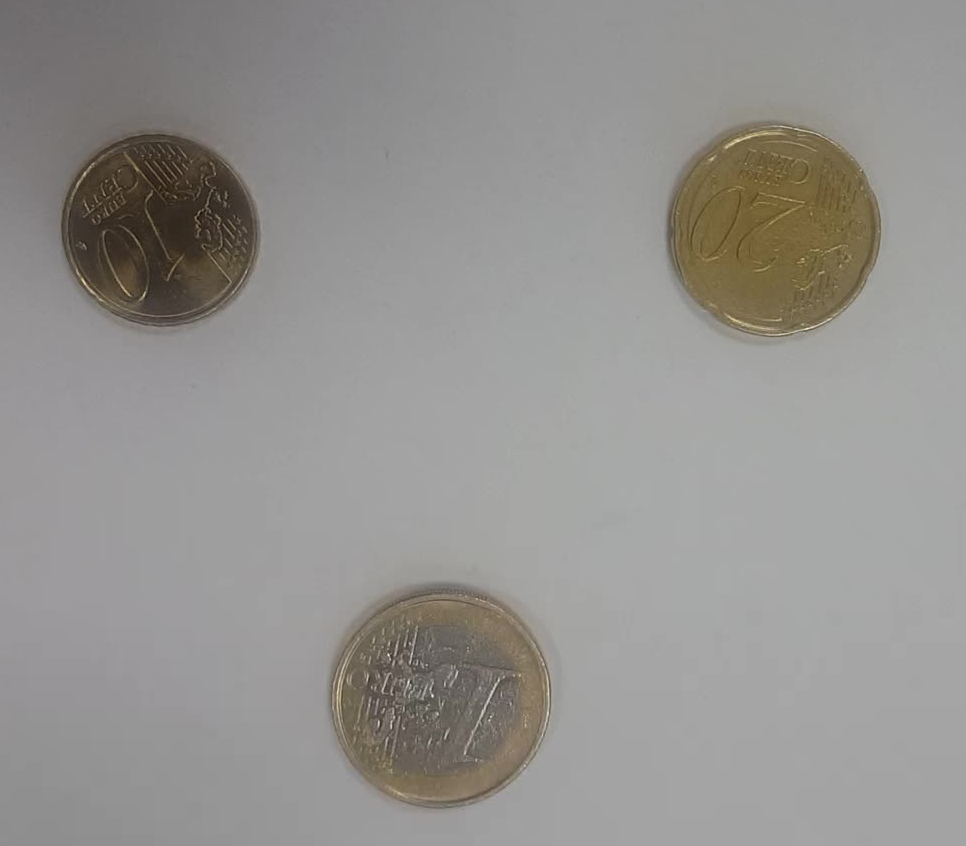
\includegraphics[scale=0.08]{inference-raw}
\caption{Example of raw image coming from the mobile camera.}
\label{fig:figure1}
\end{figure}

A python script was created to take every image and, using the Hough Transform, to extract the coins from the images. The individual images were safe in directories with the name of the classes, in this case : coin10, coin20 and con100.

These images where down-sampled. The final image size, the ones used to train the network, was 256x256 pixels. The single images for every class was safe with the following directory structure:

\dirtree{%
.1 data.
.2 coin10.
.3 coin-10-image-1.jpg.
.3 coin-10-image-2.jpg.
.2 coin20.
.3 coin-20-image-1.jpg.
.3 coin-20-image-2.jpg.
.2 coin100.
.3 coin-100-image-1.jpg.
.3 coin-100-image-2.jpg.
}

\begin{figure}[h]
\centering
\begin{subfigure}[b]{0.15\textwidth}
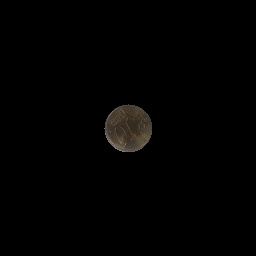
\includegraphics[scale=0.25]{output_0010_0}
\caption{10 cents}
\end{subfigure}
\begin{subfigure}[b]{0.15\textwidth}
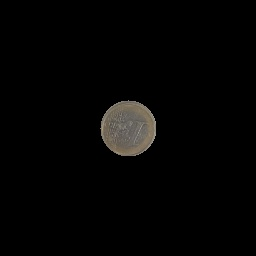
\includegraphics[scale=0.25]{output_0005_1}
\caption{20 cents}
\end{subfigure}
\begin{subfigure}[b]{0.15\textwidth}
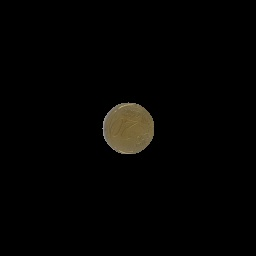
\includegraphics[scale=0.25]{output_0001_2}
\caption{1 euro}
\end{subfigure}
\label{fig:figure2}
\caption{Example images coin extracted using Hough Transform.}
\end{figure}


\section{Neural Network Trainning}

Digits tools was used to train the network. The process of training the network in digits takes two steps. The following section show the configuration for both networks: the train the dataset provided by udaciy and the original idea.

\subsection{Udacity}
\subsubsection{Create the Model}

In the first step the model from the data set, classification type, was created. The following parameters were selected:

\begin{itemize}
\item Image type[Color]: color is a  3-channel RGB image.
\item Image size(Width x Height) [256,256]: the image input will be resized to this value. 
\item Trainning Image: the folder with the structure as provided by udacity.
\item \%for validation[25\%]: the percent of image to set apart for the validation process.
\item \%for testing[5\%]: the percent of image to set apart for the test process.
\item DatasetName[udacity\-dataset]: the name of the dataset for future references.
\end{itemize}

\subsubsection{Train the Network}

The network was trained with the model and network architecture previously defined using the digits platform.

\begin{figure}[h]
\centering
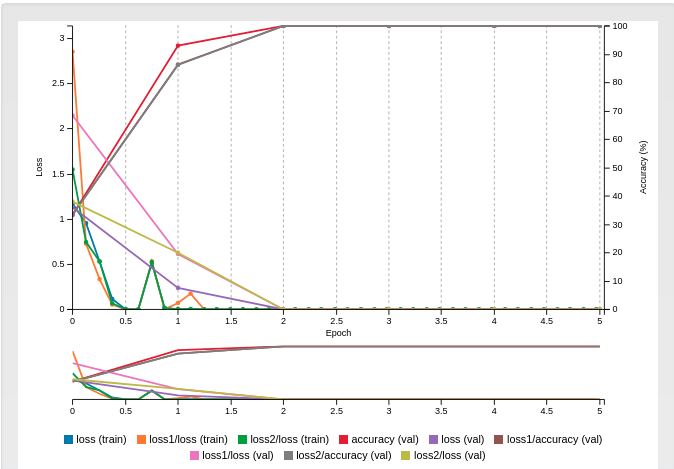
\includegraphics[scale=0.3]{trainning-chart}
\caption{Trainnig chart Udacity.}
\label{fig:figure3}
\end{figure}


\subsection{Original Idea}
\subsubsection{Create the Model}

In the first step the model from the data set, classification type, was created. The following parameters were selected:

\begin{itemize}
\item Image type[Color]: color is a  3-channel RGB image.
\item Image size(Width x Height) [256,256]: the image input will be resize to this value. Since the original image was already of this size, resizing will not take place.
\item Trainning Image: the folder with the structure describe in the previous section. 
\item \%for validation[25\%]: the percent of image to set apart for the validation process.
\item \%for testing[10\%]: the percent of image to set apart for the test process.
\item DatasetName[coin\-dataset]: the name of the dataset for future references.
\end{itemize}

\subsubsection{Train the Network}

The network was trained with the model and network architecture previously defined using the digits platform.

\begin{figure}[h]
\centering
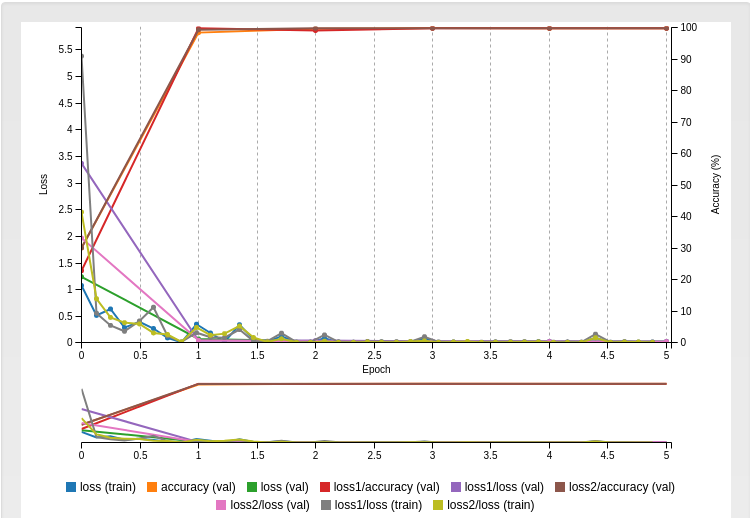
\includegraphics[scale=0.25]{trainning-chart-udacity}
\caption{Trainnig chart original idea.}
\label{fig:figure3}
\end{figure}

\section{Results}

\subsection{Udacity}

After training the network the result was evaluated, the result is on requirements.

\begin{figure}[h]
\centering
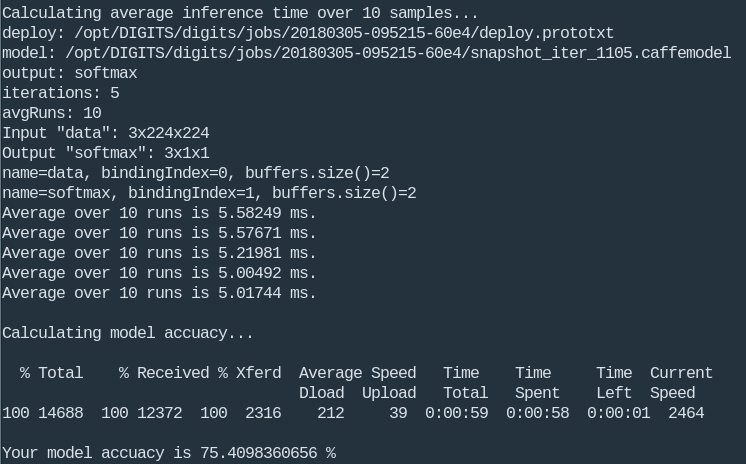
\includegraphics[scale=0.2]{udacity-evaluate}
\caption{Evaluation of the model udacity.}
\label{fig:figure4}
\end{figure}

\subsection{Original Idea}

After training the network a subset of the image reserved to test the result with the following output:

\begin{figure}[h]
\centering
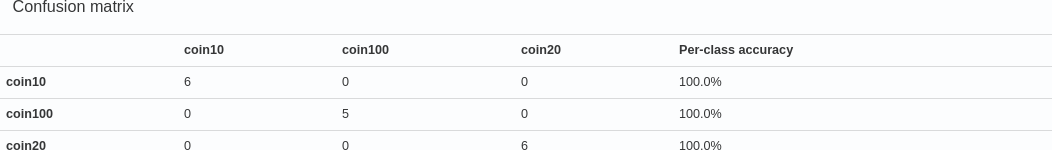
\includegraphics[scale=0.2]{confusion-matrix}
\caption{Confusion Matrix.}
\label{fig:figure5}
\end{figure}


\begin{figure}[h]
\centering
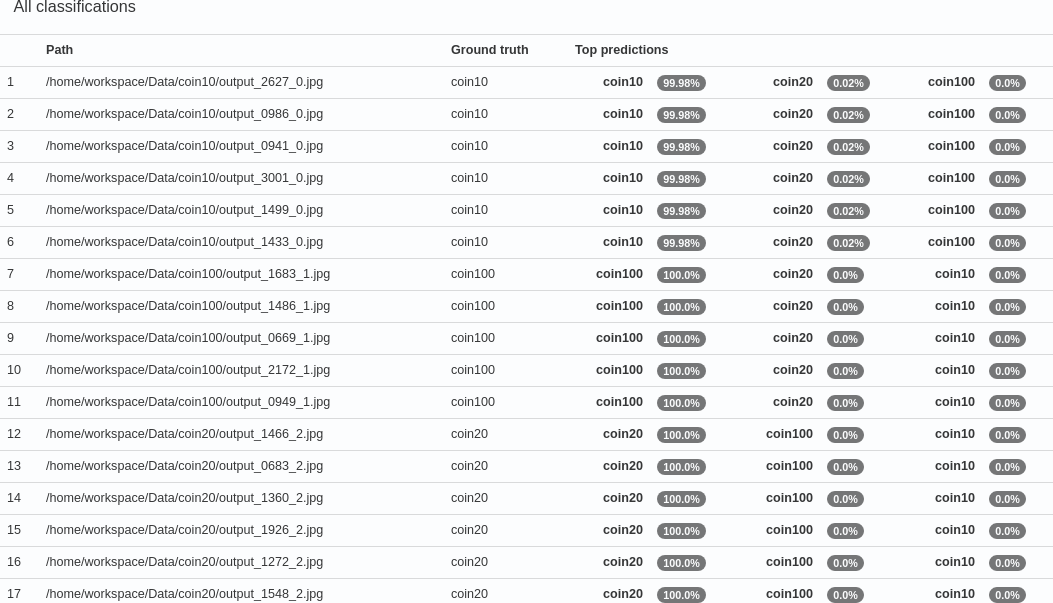
\includegraphics[scale=0.2]{classification-all}
\caption{Classification result of the network for testing images.}
\label{fig:figure6}
\end{figure}

The results of the classification were really good. 

\section{Discussion}

It has been notice during the development of this project the importance of the data collection process. In order to have a good accuracy is quite important to have a big number of samples of every class. The process of acquiring these images can be a complex and time-consuming task. The background where the object were collected is also part of the acquisition problem. In this project a mix solution, using traditional image processing techniques, Hough Transform, was used to overcame this problem. The final accuracy obtained was quite good. 

There are some parameters that must be taken in account depending on the final deployed hardware and the desire performance:accuracy, inference time, power consumption, memory use.\cite{analysisdnn}

There are relation between these parameters. For example,there are a hyperbolic relationship between the accuracy and inference time, in order to have a small increase in the accuracy the inference time will increase following a hyperbolic curve. 

For that reason the network architecture must be selected taking in consideration the specific requirements for the concrete application. Furthermore, due to the possible limitations of the hardware where the solution will be deployed, and taking in consideration the frame per seconds to be inference and the accuracy desire, the correct network architecture must be selected. 

In this project GoogleNet was selected due that the solution for both Udacity model and own model was on requirements. Furthermore, due to the possible limitations 

	
\section{Conclusion / Future work}

The accuracy of the classification process achieved was really good. Due to time constraints the classes consists only in three coin and the same side. The final number of the classes is quite bigger than that. There are eight euros coins with two side each. One of the size is common for all the European countries but the other side is country specific. This makes the process of gathering the samples more difficult and time consuming. Once the network is trained with all the coin types and size a mobile application can be used to inference the coins in the day basis. The fact that the background is extracted will make this network quite robots again different environments: coins spread out over a pub's bar or over a counter in a book store.


\begin{thebibliography}{9}
\bibliographystyle{ieeetr}

\bibitem{udacity} 
https://eu.udacity.com
\textit{Robotics Software Engineer Nanodegree program}. 

\bibitem{deeplearning} 
Adit Deshpande
\textit{The 9 Deep Learning Papers You Need To Know About}. 

\bibitem{analysisdnn} 
Alfredo Canziani, Eugenio Culurciello,Adam Paszke  
\textit{An analysis of deep neural network models for practical applications}. 
\end{thebibliography}
		
\end{document}
	
	
